\section{Compiling sparse algebra into local networks}
\label{d:sec:logical}

The physical constructions of Parts~II and~III provide controlled
families of local interactions. To use it for an arbitrary sparse system, we
must first express that system in a form compatible with those interactions.
An input matrix can have large vertex degree, signed coefficients, and
connections between variables that are far apart in any chosen geometric
layout. Its coefficients also vary with the input. We remove these freedoms
through an explicit algebraic compilation and spatial routing procedure.
The resulting matrix has positive unit off-diagonal entries, degree at most
three, and a fixed finite diagonal alphabet. Its dependence on the input is
carried by the network geometry, choices from the fixed diagonal alphabet,
and the source.

The compilation must preserve numerical information as well as exact
solutions. In particular, perturbations of auxiliary equations are part of
the residual presented by a downstream solver. We therefore bound the
inverse of every enlarged system and track arbitrary residuals through
each elimination. This supplies a stable interface between sparse algebra
and the electromagnetic construction.

\begin{proposition}[A local algebraic normal form]
\label{d:thm:logical}
Under the input assumptions~\eqref{c:eq:input}, a nonzero-source system
$Mx=b$ can be transformed deterministically into
\begin{equation}
    \Gamma z=g_\Gamma
    \label{d:eq:logical-normal-form}
\end{equation}
with the following properties. The matrix $\Gamma$ is real symmetric and
supported on a subgraph of the three-dimensional unit cubic lattice. Its
graph degree is at most three, every nonzero off-diagonal entry equals
$+1$, and its diagonal belongs to a fixed finite subset of $[-3,3]$.
Moreover,
\begin{equation}
    \norm{\Gamma}_2\le 7,
    \qquad
    \norm{\Gamma^{-1}}_2\le \overline K,
    \label{d:eq:logical-norms}
\end{equation}
where $\overline K$ is an explicit polynomial bound in $m$.
The bounding rectangular box has $O((m\log m)^{3/2})$ lattice sites.
The source coordinates have $O(\log m)$ bits, and a prescribed
inverse-polynomial relative residual for~\eqref{d:eq:logical-normal-form}
suffices for coordinate selection, rounding, and scalar rescaling to
recover an answer to $Mx=b$ at the requested relative residual.
Construction and decoding, including writing the full occupancy of the
bounding box, require $\Ot(m^{3/2})$ bit operations.
\end{proposition}

The constants in this proposition depend only on the fixed input constants $c_\kappa,c_\eta,B_{\rm in}$.
The construction does not call a solver for the original system. We give
the main transformations here and prove their quantitative claims in
Sections~\ref{d:app:logical}--\ref{d:app:logical-residual}.

\subsection{Short coefficients through a stable arithmetic circuit}

Let $P=m^{\lceil c_\kappa\rceil+1}$ and
$\eta_0=m^{-\lceil c_\eta\rceil}$. For $b\ne0$, define
\begin{equation}
 a_M=\max_{i,j}|M_{ij}|,\qquad \nu_M=\norm{b}_\infty,
 \qquad F=M/(ma_M),\qquad g=b/\nu_M.
 \label{d:eq:logical-normalization}
\end{equation}
Then $\norm{F}_2\le1$, $\sigma_{\min}(F)\ge P^{-1}$, and
$1\le\norm{g}_2\le\sqrt m$. Solving $Fu=g$ gives
$x=(\nu_M/(ma_M))u$. Round the existing entries of $F$ to a dyadic grid
of spacing $2^{-N_{\rm r}}\le\eta_0/(64mP)$, without introducing entries outside
the original sparsity pattern. The rounded matrix $\widehat F$ satisfies
\begin{equation}
 \norm{\widehat F-F}_2\le \frac{\eta_0}{64P},
 \qquad \norm{\widehat F^{-1}}_2\le2P,
 \qquad N_{\rm r}=O(\log m).
 \label{d:eq:logical-rounding}
\end{equation}

We express multiplication by each dyadic coefficient through binary
Horner evaluation. Copy trees give a separate occurrence of an input to
each nonzero coefficient bit, and binary addition trees sum the resulting
terms within each row. A sign gate implements each coefficient's sign.
The equations defining these gates, together with the output equations,
form a square system
\begin{equation}
 \Gamma_{\rm c}\begin{pmatrix}u\\w\end{pmatrix}=g_{\rm c}
 \label{d:eq:logical-circuit}
\end{equation}
of size $S\le6m(N_{\rm r}+1)$. Every coefficient of $\Gamma_{\rm c}$ belongs to
$\{0,\pm1,\pm\tfrac12\}$, and each row and column has at most three
nonzero entries. In particular, $\norm{\Gamma_{\rm c}}_2\le3$.

The circuit is arranged so that an auxiliary perturbation cannot be
amplified exponentially by repeated branching and recombination. If its
gate equations are $T_{\rm g}w-B_{\rm g}u=\rho_{\rm aux}$, then $T_{\rm g}$ is unit lower triangular
and each entry of $T_{\rm g}^{-1}$ is a sum over directed paths. Branching occurs
only in the initial copy trees; after leaving a copy tree, a path follows
a Horner chain, a sign gate, and a row-sum tree without further branching.
There are at most $S$ paths between any two gates. Consequently,
\begin{equation}
 \norm{T_{\rm g}^{-1}}_2\le S^2,
 \qquad \norm{\Gamma_{\rm c}^{-1}}_2\le16PS^4=:Q_{\rm c}.
 \label{d:eq:logical-circuit-stability}
\end{equation}
More specifically, for any approximate solution of the circuit equations,
\begin{equation}
 \norm{\widehat F u-g}_2
 \le \sqrt n\bigl((S+1)^2+1\bigr)
      \norm{\Gamma_{\rm c}(u,w)-g_{\rm c}}_2.
 \label{d:eq:logical-circuit-residual}
\end{equation}
This estimate treats all gate equations as potentially inexact. It is the
property needed when the circuit is later recovered from an approximate
electromagnetic field.

\subsection{Signed algebra with positive unit edges}

Symmetrization gives
\begin{equation}
 \Gamma_0=\begin{pmatrix}0&\Gamma_{\rm c}\\\Gamma_{\rm c}^\top&0\end{pmatrix},
 \qquad\text{with source }\begin{pmatrix}g_{\rm c}\\0\end{pmatrix}.
 \label{d:eq:logical-symmetrization}
\end{equation}
The singular values of $\Gamma_{\rm c}$ become the absolute eigenvalues of $\Gamma_0$.
Thus this step preserves the relevant norm and inverse-norm bounds,
while a block of its residual is exactly the circuit residual.

To replace a signed edge of weight $w_e\in\{\pm1,\pm\tfrac12\}$,
introduce a mediator connected to its two endpoints by edges of weight
$+1$. Give that mediator diagonal $-1/w_e$, and give each original vertex
the negative sum of its incident old weights. If $\mathcal I$ is the unsigned
incidence matrix, $(D_{\rm med})_{ee}=-1/w_e$, and $D_{\rm end}$ is this endpoint diagonal,
the enlarged matrix is
\begin{equation}
 \Gamma_+=\begin{pmatrix}D_{\rm end}&\mathcal I\\\mathcal I^\top&D_{\rm med}\end{pmatrix},
 \qquad D_{\rm end}-\mathcal ID_{\rm med}^{-1}\mathcal I^\top=\Gamma_0.
 \label{d:eq:logical-sign-mediators}
\end{equation}
The identity in~\eqref{d:eq:logical-sign-mediators} explains how signs are
represented using positive unit edges: they appear in the effective
interaction after mediator elimination. The mediator diagonals belong to
$\{-2,-1,1,2\}$, while endpoint diagonals are half-integers in $[-3,3]$.
The degree remains at most three.

The graph of $\Gamma_+$ is bipartite, with original vertices on one side and
mediators on the other. It has at most $S_+=5S$ vertices. Since
$\norm{\mathcal I}_2\le\sqrt6$ and $\norm{D_{\rm med}^{-1}}_2\le1$, block factorization
gives
\begin{equation}
 \norm{\Gamma_+^{-1}}_2\le16Q_{\rm c}=:Q_+.
 \label{d:eq:logical-positive-inverse}
\end{equation}
Eliminating a mediator residual amplifies its norm by less than four.
Thus neither the sign conversion nor symmetrization loses polynomial
control.

\subsection{Routing the network in three dimensions}

We next embed a subdivision of this bounded-degree bipartite graph in a
cubic lattice. Each incidence receives its own port in a square array.
The two ports of each edge are routed to a designated adjacent pair at
the top of a three-dimensional box. A row--column--row permutation
schedule realizes all these assignments. The schedule is obtained by
recursively splitting even-regular bipartite multigraphs into perfect
matchings and using adjacent odd--even transposition sorting within rows
and columns. Each swap occupies a fixed-size lattice box, with two
vertex-disjoint paths inside it.

For a power of two $\ell_{\rm p}$ with $2\sqrt{S_+}\le\ell_{\rm p}<4\sqrt{S_+}$, the construction
uses a box with all three side lengths $O(\ell_{\rm p})$. Each routed edge has length
at most $\ell_w=1024\ell_{\rm p}$. The box therefore contains $O(S_+^{3/2})$ sites,
including the sites not occupied by a path. This accounting is the source
of the exponent $3/2$ in the construction. The volume $O(S_+^{3/2})$
matches the classical bound for realizing bounded-degree networks in
three dimensions~\citep{KolmogorovBarzdin1967,LeightonRosenberg1986}.

Path length also controls the sign of the effective endpoint interaction.
The bipartition permits endpoints of opposite lattice parity. We then add
a local two-edge detour whenever needed so that every path length is
$1$ modulo $4$. Put zero diagonal on the internal vertices and $+1$ on
every path edge. If a path has $4j$ internal vertices, the inverse of its
internal adjacency matrix has vanishing endpoint diagonal entries and
far-corner entry $-1$. Its Schur complement is therefore exactly a
positive unit endpoint edge, with no diagonal correction. The routed
matrix $\Gamma$ has $\Gamma_+$ as its exact Schur complement.

The same calculation yields the explicit bound
\begin{equation}
 \overline K=9\ell_w^2(Q_++\ell_w)
 \quad\text{with}\quad
 \norm{\Gamma^{-1}}_2\le\overline K.
 \label{d:eq:logical-final-inverse}
\end{equation}
Since $S=O(m\log m)$ and $\ell_w=O(\sqrt S)$, this is polynomial in $m$.
The geometric layout uses $\Ot(m^{3/2})$ volume and bit operations.
We do not know whether this routing exponent is optimal.

\subsection{Residuals and decoding}

Let
\begin{equation}
 T_{\rm res}=4n\bigl((S+1)^2+1\bigr)(1+2\ell_w),
 \qquad \eta_{\rm res}=\frac{\eta_0}{16T_{\rm res}}.
 \label{d:eq:logical-tolerance}
\end{equation}
Eliminating internal path vertices, eliminating sign mediators, selecting
the circuit block, and eliminating gate variables transfers a relative
$\eta_{\rm res}$ residual for $\Gamma$ into an error at most
$\eta_0\norm{g}_2/16$ for $\widehat F u=g$. Equation
\eqref{d:eq:logical-rounding} then controls the difference between
$\widehat F$ and $F$. Rounding the selected input coordinates on a grid
of spacing $\eta_0/(16m)$ leaves the normalized residual below
$\eta_0\norm{g}_2/4$. Scalar rescaling by $\nu_M/(ma_M)$ produces the
required answer to the original system.

The decoder uses coordinate restriction and short rational arithmetic.
The selected coordinates have polynomial magnitude, so their required
integer and fractional precision is $O(\log m)$ bits. Every auxiliary
variable, path vertex, empty site in the bounding box, and decoding
operation has been included in the resource estimate. The output of this
section is thus a quantitative normal form suitable for the finite
Maxwell assembly.

\begin{figure}[tbp]
\centering
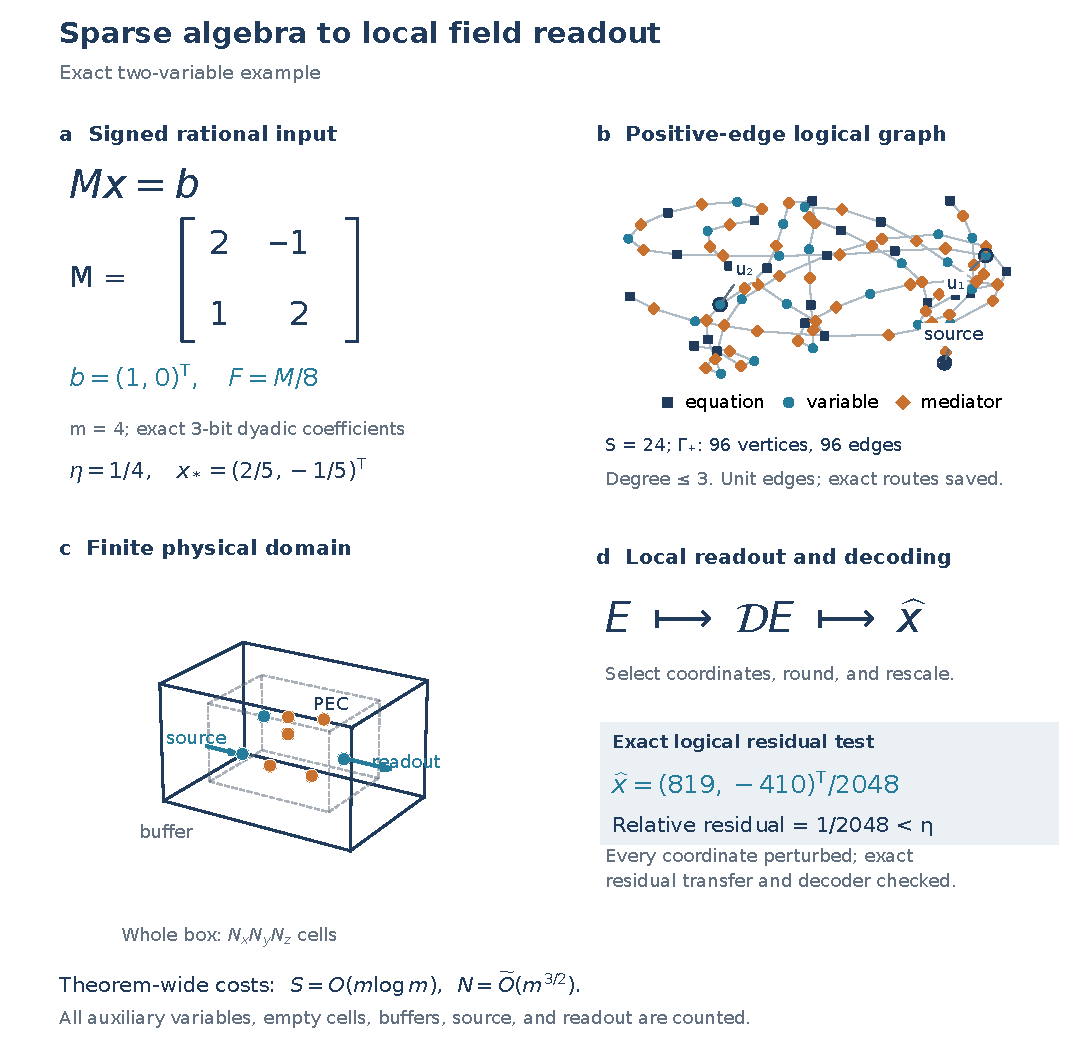
\includegraphics[width=\linewidth]{figures/si/logical_translation.pdf}
\caption{An exact sparse-algebra example and the schematic physical
translation. (a) The signed nonsymmetric matrix is normalized to
$F=M/8$ with no coefficient rounding error. (b) The actual compiled
circuit has $S=24$ variables; symmetrization and sign mediators give the
shown $\Gamma_+$ graph with 96 vertices and 96 positive unit edges, degree
at most three, and fixed half-integer diagonals. Its verified cubic
routing, supplied as exact figure data, has 760\,320 occupied lattice
sites in a $505\times169\times3105$ bounding box containing
264\,996\,225 sites in total. (c) Scalar dielectric defects, the complete
PEC box, buffer, source, and local readout are schematic. The physical construction counts all
$N_xN_yN_z$ cells. (d) An exact perturbation of every logical coordinate,
in place of a computed Maxwell field, passes the prescribed logical
residual tolerance; coordinate selection,
rounding, and rescaling return $\widehat x=(819,-410)^\top/2048$ with
relative source-system residual $1/2048<\eta=1/4$.}
\label{d:fig:overview}
\end{figure}

\subsection{The interface used by the continuum back end}
The continuum assembly in Part~II uses the following form of
Proposition~\ref{d:thm:logical}, with a logical tolerance
$\eta_\Gamma$ fixed in advance. Sections~\ref{d:app:logical}--\ref{d:app:logical-residual}
prove it; Remark~\ref{si:rem:continuum-compiler} records the
parameter-specific details.

\begin{lemma}[Logical interface]
\label{c:lem:logical}
In $\tO(m^{3/2})$ bit operations one constructs a real symmetric matrix
$\Gamma$ on a subgraph of the unit cubic lattice, of degree at most three,
with positive unit edges and half-integer diagonals in $[-3,3]$.
It has $\norm\Gamma\le7$, an explicit polynomial bound
$\norm{\Gamma^{-1}}\le \overline K$, and a source $g$ with
$\norm g_\infty=1$ and at most $m$ nonzero entries. All three side lengths
of its bounding box are $O(\sqrt{m\log(2+m)})$.
An explicit $\ee>0$, with $\ee^{-1}$ polynomial in $m$, has the property
that every $z$ satisfying
$\norm{\Gamma z-g}\le\ee\norm g$ decodes by coordinate selection,
rounding, and rational rescaling to~\eqref{c:eq:target}.

The complete list of parameters is
\begin{align}
 P&=m^{\lceil c_\kappa\rceil+1},\qquad \eta_0=m^{-\lceil c_\eta\rceil},
 \qquad 2^{-N_{\rm r}}\le\eta_0/(64mP),\\
 S&\le6m(N_{\rm r}+1),\quad S_+\le5S,\quad
 2\sqrt{S_+}\le\ell_{\rm p}<4\sqrt{S_+},\quad \ell_{\rm p}\text{ a power of two},\\
 \ell_w&=1024\ell_{\rm p},\quad Q_{\rm c}=16PS^4,\quad Q_+=16Q_{\rm c},\\
 \overline K&=9\ell_w^2(Q_++\ell_w),\qquad
 T_{\rm res}=4n\bigl((S+1)^2+1\bigr)(1+2\ell_w),\notag\\
 \eta_*&=\min\left\{\frac12,
 \frac{\eta_0}{\max\{1,T_{\rm res}\}\max\{1,m^2\}}\right\},
 \qquad \ee=\eta_*/16.                         \label{c:eq:logicalparameters}
\end{align}
Thus $T_{\rm res}\ee\le\eta_0/16$. The factor $1/16$ reserves the
logical residual margin. The factor $\max\{1,m^2\}$ is a spare margin:
the continuum chain budgets its absolute readout errors separately,
through $h_y$ in~\eqref{c:eq:momentaccuracy} and $e_0$
in~\eqref{c:eq:e0}. All choices use rational arithmetic.
A bounding box has at most $2^{17}\ell_{\rm p}^3$ sites. These include its empty
sites, not only its graph vertices.
\end{lemma}

\section{A stable compiler for sparse linear systems}
\label{d:app:logical}

We prove Proposition~\ref{d:thm:logical} with explicit parameters. All
norms in this section are Euclidean operator or vector norms unless a
subscript states otherwise. The case $b=0$ is answered by $x=0$; bounded
input sizes can be handled by a fixed finite computation. We therefore
assume $m\ge2$ and $b\ne0$.

\subsection{Normalization and perturbation bounds}

Set $P=m^{\lceil c_\kappa\rceil+1}$,
$\eta_0=m^{-\lceil c_\eta\rceil}$, and use the normalization in
\eqref{d:eq:logical-normalization}. Since
\begin{equation}
 a_M\le\norm{M}\le\norm{M}_{\mathrm F}\le\sqrt m\,a_M,
 \qquad \sigma_{\min}(M)\ge a_M m^{-c_\kappa},
\end{equation}
we have $\norm{F}\le1$ and $\norm{F^{-1}}\le P$.
The vector $g$ has infinity norm one and at most $m$ coordinates.
Choose an integer $N_{\rm r}\ge1$ such that
$2^{-N_{\rm r}}\le\eta_0/(64mP)$ and round each existing nonzero of $F$
to its nearest multiple of $2^{-N_{\rm r}}$, with a fixed tie rule. Delete entries
that become zero. Then
\begin{equation}
 \norm{\widehat F-F}
 \le\norm{\widehat F-F}_{\mathrm F}
 \le\sqrt m\,2^{-N_{\rm r}}/2\le\eta_0/(64P).
 \label{d:eq:app-dyadic-perturbation}
\end{equation}
In particular,
$\norm{F^{-1}(\widehat F-F)}\le1/64$.
The Neumann series for
$[I+F^{-1}(\widehat F-F)]^{-1}$ gives
$\norm{\widehat F^{-1}}\le2P$.
Each coefficient has $N_{\rm r}=O_{c_\kappa,c_\eta}(\log m)$ fractional bits. Normalization
and rounding can be performed independently on each short rational
input entry, in $O(m\operatorname{polylog}m)$ bit operations; a common
denominator across all entries is unnecessary.

\subsection{An acyclic circuit with a polynomial inverse}

Write each nonzero absolute dyadic coefficient as
\begin{equation}
 |\widehat F_{ij}|=\sum_{a=1}^{N_{\rm r}} t_{ij,a}2^{-a},
 \qquad t_{ij,a}\in\{0,1\}.
\end{equation}
For each original input variable $u_j$, build a binary copy tree with
one leaf for each nonzero bit occurrence referring to $u_j$. An input
or copy output has at most two later uses. If there is only one use,
the original input can supply it directly. Nonsingularity of
$\widehat F$ ensures that every input has a use.

For each coefficient, use the Horner equations
\begin{equation}
 v_{N_{\rm r}+1}=0,\qquad
 v_a=\tfrac12 v_{a+1}
       +\tfrac12 t_{ij,a}u_{j,a},\qquad a=N_{\rm r},N_{\rm r}-1,\ldots,1.
 \label{d:eq:app-horner}
\end{equation}
The value $v_{N_{\rm r}+1}=0$ is a constant and not an additional variable.
Each nonzero bit uses its designated copy-tree leaf. A sign gate
multiplies $v_1$ by $\operatorname{sign}(\widehat F_{ij})$, and a binary
addition tree sums the terms of each row. Let its output be $o_i$.
There is at least one term per row. The defining gate equations and
the $n$ equations $o_i=g_i$ give the square system
$\Gamma_{\rm c}(u,w)=g_{\rm c}$.

There are at most $mN_{\rm r}$ bit occurrences. The copy trees use at most
$2mN_{\rm r}$ gates, the Horner chains at most $mN_{\rm r}$, sign gates at most $m$,
and row additions at most $m$. Including original inputs gives
\begin{equation}
 S=n+\dim w\le6m(N_{\rm r}+1).
\end{equation}
Every equation has at most three coefficients of absolute value at
most one. Every variable occurs in its defining equation, if present,
and at most two later uses. Thus the row and column absolute sums of
$\Gamma_{\rm c}$ are at most three and $\norm{\Gamma_{\rm c}}\le3$.

In topological order, the auxiliary equations take the form
$T_{\rm g}w-B_{\rm g}u=\rho_{\rm aux}$, where $T_{\rm g}$ is unit lower triangular. Each row of
$B_{\rm g}$ has at most one nonzero and each column at most two, so
$\norm{B_{\rm g}}\le2$. If $R_{\rm g}$ selects the distinct row outputs, then
$\norm{R_{\rm g}}\le1$ and
\begin{equation}
 \widehat F=R_{\rm g}T_{\rm g}^{-1}B_{\rm g}.
 \label{d:eq:app-circuit-factorization}
\end{equation}
The inverse $T_{\rm g}^{-1}$ is a finite weighted-path expansion. Edge weights
have absolute value at most one. Within a copy tree there is a unique
path between any compatible pair of gates. A path that leaves a copy
tree is determined by its exit leaf and then has at most one
continuation: Horner chains, sign gates, and addition trees all have
outdegree at most one. Hence at most $S$ paths connect any pair of
auxiliary gates. Every inverse entry has absolute value at most $S$,
which gives $\norm{T_{\rm g}^{-1}}\le S^2$.

For an arbitrary right-hand side $\rho=(\rho_{\rm out},\rho_{\rm aux})$,
eliminating $w$ in the equations defining $\Gamma_{\rm c}^{-1}\rho$ yields
\begin{equation}
 \widehat F u=\rho_{\rm out}-R_{\rm g}T_{\rm g}^{-1}\rho_{\rm aux}.
\end{equation}
Therefore
\begin{align}
 \norm{u}&\le2P(1+S^2)\norm{\rho}\le4PS^2\norm{\rho},\\
 \norm{w}&\le S^2(2\norm{u}+\norm{\rho})
             \le9PS^4\norm{\rho}.
\end{align}
Combining these estimates proves
$\norm{\Gamma_{\rm c}^{-1}}\le16PS^4=Q_{\rm c}$.
For residual transport we use an explicit coordinate bound. Put
$e_{\rm c}=\norm{\Gamma_{\rm c}(u,w)-g_{\rm c}}$. Every gate residual has magnitude at most $e_{\rm c}$.
A copy leaf differs from its input by at most $Se_{\rm c}$. In each row expression,
weights have magnitude at most one and every occurrence has its own leaf.
Induction through its addition and scaling gates bounds the output error
by the number of gates times $e_{\rm c}$, plus the sum of its leaf errors. There
are at most $S$ gates and $S+1$ leaves, so this is at most $(S+1)^2e_{\rm c}$.
The output equation contributes one further $e_{\rm c}$ per row. Taking the
Euclidean norm over the $n$ rows proves
\eqref{d:eq:logical-circuit-residual}. The bound includes residuals in
every auxiliary equation.

\subsection{Symmetrization and sign mediators}

Form $\Gamma_0$ and its source as in~\eqref{d:eq:logical-symmetrization}.
Its graph is bipartite and has $2S$ vertices and at most $3S$ edges.
Direct multiplication gives
$\Gamma_0^2=\operatorname{diag}(\Gamma_{\rm c}\Gamma_{\rm c}^\top,\Gamma_{\rm c}^\top\Gamma_{\rm c})$, so
$\norm{\Gamma_0}=\norm{\Gamma_{\rm c}}$ and
$\norm{\Gamma_0^{-1}}=\norm{\Gamma_{\rm c}^{-1}}$.
For a residual solution $(v,(u,w))$, the first block of the residual
is $\Gamma_{\rm c}(u,w)-g_{\rm c}$ and needs no amplification to be recovered.

For each edge $e=\{i,j\}$ with weight $w_e$, introduce a mediator with
diagonal $(D_{\rm med})_{ee}=-1/w_e$. Let $\mathcal I$ be the unsigned incidence matrix of
the old graph and set $(D_{\rm end})_{ii}=-\sum_{e\ni i}w_e$. Since
$(D_{\rm med})_{ee}^{-1}=-w_e$, the diagonal entries of $\mathcal ID_{\rm med}^{-1}\mathcal I^\top$ equal
$-\sum_{e\ni i}w_e$, and its off-diagonal $ij$ entry is $-w_e$.
It follows that $D_{\rm end}-\mathcal ID_{\rm med}^{-1}\mathcal I^\top=\Gamma_0$ exactly.

The enlarged graph has $S_+\le5S$ vertices, degree at most three, and
positive unit edges. Its endpoint diagonals lie in
$\{j/2:-6\le j\le6\}$; its mediator diagonals lie in
$\{-2,-1,1,2\}$. The incidence bounds give
$\norm{\mathcal I}\le\sqrt{\norm{\mathcal I}_1\norm{\mathcal I}_\infty}\le\sqrt6$ and
$\norm{D_{\rm med}^{-1}}\le1$.
The factorization
\begin{equation}
 \Gamma_+=
 \begin{pmatrix}I&\mathcal ID_{\rm med}^{-1}\\0&I\end{pmatrix}
 \begin{pmatrix}\Gamma_0&0\\0&D_{\rm med}\end{pmatrix}
 \begin{pmatrix}I&0\\D_{\rm med}^{-1}\mathcal I^\top&I\end{pmatrix}
\end{equation}
implies
\begin{equation}
 \norm{\Gamma_+^{-1}}
 \le(1+\sqrt6)^2\max(1,Q_{\rm c})\le16Q_{\rm c}=Q_+.
\end{equation}
The source is $(g_{\rm c},0,0)$. Subtracting $\mathcal ID_{\rm med}^{-1}$ times the mediator
residual from the endpoint residual shows that the recovered $\Gamma_0$
residual has norm at most
$(1+\sqrt6)\norm{\rho_{\Gamma_+}}<4\norm{\rho_{\Gamma_+}}$.

\section{Explicit three-dimensional routing}
\label{d:app:routing}

\begin{lemma}[A counted cubic embedding]
\label{d:lem:cubic-routing}
A bipartite graph with $S_+$ vertices and degree at most three admits an
explicit subdivision in a rectangular unit cubic lattice box containing
$O(S_+^{3/2})$ sites. Distinct edge paths meet only at common graph
endpoints. For a power of two $\ell_{\rm p}$ with
$2\sqrt{S_+}\le\ell_{\rm p}<4\sqrt{S_+}$, every path has length at most $1024\ell_{\rm p}$
and length congruent to $1$ modulo $4$. The paths and the full bounding
box can be written in $O(S_+^{3/2}\log S_+)$ bit operations.
\end{lemma}

\begin{proof}
Put $\ell_{\rm p}=2^{1+\lceil(\log_2S_+)/2\rceil}$, twice the least power of two whose square is at least $S_+$.
Place the graph vertices in an $(\ell_{\rm p}/2)$ by $(\ell_{\rm p}/2)$ array and allocate a $2$ by
$2$ tile of an $\ell_{\rm p}$ by $\ell_{\rm p}$ port array to each vertex. Three positions in
the tile serve its incidences; unused positions are dummy ports. Assign
the two incidence tokens of each edge to one designated horizontal
pair of adjacent target ports. There are $\ell_{\rm p}^2/2\ge2S_+$ pairs, whereas
the graph has at most $3S_+/2$ edges. Assign dummy tokens to the remaining
targets to complete a permutation of all $\ell_{\rm p}^2$ ports.

Construct a bipartite multigraph whose two vertex sets are the $\ell_{\rm p}$
source rows and the $\ell_{\rm p}$ target rows, with one edge per token. This graph
is $\ell_{\rm p}$-regular. At an even-degree stage, pair consecutive incidences at
each source vertex and at each target vertex. The pairings define
fixed-point-free involutions $\iota_1,\iota_2$ on the tokens. Their alternating
components are even cycles, including the two-token case. For $\varpi=\iota_1\iota_2$,
the $\varpi$-orbits of $i$ and $\iota_1(i)$ are the two disjoint halves of one
component. Color $i$ according to which half has the smaller token label.
Both pairings reverse this color, so each color receives half the
incidences at every vertex.

The orbit minima are computed by stored arrays, not repeated traversal.
With $N_t$ tokens, initialize $j_0(i)=\varpi(i)$ and $\mu_0(i)=i$ and perform
\[
 j_{t+1}(i)=j_t(j_t(i)),\qquad
 \mu_{t+1}(i)=\min\{\mu_t(i),\mu_t(j_t(i))\}.
\]
Each pass reads the previous arrays and writes fresh arrays. After $t$
passes, $j_t(i)=\varpi^{2^t}(i)$ and $\mu_t(i)$ is the least label in the first
$2^t$ orbit positions. Thus $\lceil\log_2 N_t\rceil$ passes suffice.
The final comparison is $\mu_t(i)<\mu_t(\iota_1(i))$. Split the incidence lists
by this color and recurse until degree one; this gives $\ell_{\rm p}$ perfect
matchings. Each recursion level has $\ell_{\rm p}^2$ tokens in total and needs
$O(\ell_{\rm p}^2\log\ell_{\rm p})$ array operations. Across all levels the cost is
$O(\ell_{\rm p}^2(1+\log\ell_{\rm p})^2)$ array operations, including the pairings and
materialized output lists. Token labels have $O(\log\ell_{\rm p})$ bits.
Consequently the coloring bit cost is $O(\ell_{\rm p}^2(1+\log\ell_{\rm p})^3)$, which is
$O(\ell_{\rm p}^3\log\ell_{\rm p})$ after adjusting a fixed constant for small $\ell_{\rm p}$.

Give each token the color $j\in\{0,\ldots,\ell_{\rm p}-1\}$ of its matching.
First permute tokens within each source row so that color $j$ lies in
column $j$. Second, permute tokens within each column by their target
row. Third, permute tokens within each target row by their target
column. Each step is a collection of line permutations: a matching
contains each source and target row once, and the target ports were
assigned bijectively.

Each line permutation can be implemented by odd--even transposition
sort, i.e., parallel layers of adjacent comparisons that alternate
between odd and even positions. This network sorts any line of length
$\ell_{\rm p}$ in $\ell_{\rm p}$ layers~\citep[Section~5.3.4]{knuth1998}. We use $2\ell_{\rm p}$
layers in each of the three phases, giving $6\ell_{\rm p}$ layers in total.

To realize these layers geometrically, put port $(i,j)$ at
$(16i,16j,0)$ and allocate height $16$ per layer. A stationary token
travels vertically. For a swap between ports $(0,0,0)$ and $(16,0,0)$,
use the following two polygonal paths, filling each segment with unit
lattice edges:
\begin{align*}
 \mathcal P_A:\ &(0,0,0),(0,0,4),(0,4,4),(16,4,4),\\
       &(16,4,12),(16,0,12),(16,0,16),\\
 \mathcal P_B:\ &(16,0,0),(16,0,8),(16,-4,8),(0,-4,8),\\
       &(0,-4,12),(0,0,12),(0,0,16).
\end{align*}
Both paths have length $40$. Their vertices are disjoint, their
interiors lie strictly between the two slab faces, and their only
face points are the four ports. Translate this gadget for row swaps
and interchange the first two coordinates for column swaps. In a
single layer, swapped pairs are disjoint; row or column spacing is
$16$, while the sideways excursion has magnitude at most $4$.
Thus different swap boxes and stationary token paths are disjoint.
Successive layers meet only at their ports, occupied by a permutation
of the tokens.

After the final layer, extend each real incidence vertically by $16$
and join each designated adjacent pair by a horizontal segment at that
height. These segments are disjoint. Discard all dummy-token paths.

It remains to connect the incidences belonging to each graph vertex.
For tile $(i,j)$, its three port positions
are $(32i,32j,0)$, $(32i+16,32j,0)$, and $(32i,32j+16,0)$.
Place the graph vertex at $(32i,32j,-16)$ for one
bipartition and at $(32i,32j,-15)$ for the other. Connect to the first port
vertically. For either other port, first travel horizontally at the
height of the vertex, then vertically. These three arms meet only at their graph
vertex; different bottom stars lie in disjoint tiles. An original
edge now follows its first bottom arm and token trajectory, its top
pairing segment, and the reversed second trajectory and bottom arm.
It is simple, and two such paths intersect only at a shared endpoint.

The two bipartitions have opposite lattice parity, so each complete
edge path has odd length. For a path of length $3$ modulo $4$, replace
the unit segment from height $-8$ to $-7$ in one of its incidence arms
by a three-edge detour displaced one unit in the positive first
coordinate. These vertical arms are distinct and at least $16$ apart.
The detour lies above the bottom spokes and below the sorting layers,
so it is disjoint from all other paths. It adds two to the length,
giving $1$ modulo $4$.

An incidence trajectory has length at most $40\cdot6\ell_{\rm p}=240\ell_{\rm p}$. The two bottom
arms total at most $64$, the two top extensions contribute $32$, the
top pairing contributes $16$, and the parity detour contributes at
most two. Hence every edge length is at most
$480\ell_{\rm p}+114\le1024\ell_{\rm p}$. All coordinates fit in a box with side lengths
at most $16\ell_{\rm p}+9$, $16\ell_{\rm p}+9$, and $96\ell_{\rm p}+33$, whose number of lattice sites
is $O(\ell_{\rm p}^3)=O(S_+^{3/2})$. Token sorting uses $O(\ell_{\rm p}^3)$ comparisons on
$O(\log S_+)$-bit keys, and explicit path output uses $O(S_+\ell_{\rm p})$ steps.
Writing the entire occupancy array also costs $O(\ell_{\rm p}^3)$ word operations.
This proves all claims.
\end{proof}

\section{Residual transfer through the routed system}
\label{d:app:logical-residual}

Apply Lemma~\ref{d:lem:cubic-routing} to $\Gamma_+$. On a path of length
$4j+1$, keep all edge weights equal to $+1$ and give its $4j$ internal
vertices zero diagonal. Denote their adjacency matrix by $\Gamma_{4j}$.
For $j\ge1$, the recurrence
\begin{equation}
 v_{a-1}+v_{a+1}=\rho_a,\qquad v_0=v_{4j+1}=0,
\end{equation}
expresses the even coordinates as alternating sums of odd right-hand
side entries from the left, and the odd coordinates as alternating
sums of even entries from the right. Every inverse entry is $0$ or
$\pm1$, and
\begin{equation}
 (\Gamma_{4j}^{-1})_{1,1}=(\Gamma_{4j}^{-1})_{4j,4j}=0,
 \quad (\Gamma_{4j}^{-1})_{1,4j}=-1,
 \quad \norm{\Gamma_{4j}^{-1}}\le4j.
 \label{d:eq:app-wire-inverse}
\end{equation}
The endpoint Schur complement therefore has zero diagonal correction
and off-diagonal contribution $+1$. For $j=0$, the direct edge is
retained. Eliminating all internal path vertices recovers $\Gamma_+$
exactly.

Let $D_{\rm wire}$ be the block diagonal matrix of all nonempty
internal paths and $\mathcal I_{\rm wire}$ the endpoint-to-internal incidence
block. With $\ell_w=1024\ell_{\rm p}$,
\begin{equation}
 \norm{D_{\rm wire}^{-1}}\le\ell_w,
 \qquad \norm{\mathcal I_{\rm wire}}\le\sqrt3<2.
\end{equation}
The second estimate follows because an endpoint has at most three
incidences, while an internal vertex next to an endpoint belongs to
only that endpoint. A nonempty internal path has at least four
vertices. Block factorization, as in the mediator step, gives
\begin{equation}
 \norm{\Gamma^{-1}}
 \le (1+2\ell_w)^2\max(Q_+,\ell_w)
 \le9\ell_w^2(Q_++\ell_w)=\overline K.
\end{equation}
All retained diagonals have magnitude at most three and every row has
at most three unit edges, so $\norm{\Gamma}\le6\le7$.

The source $g_\Gamma$ is the circuit source with zeros appended in all
other coordinates, and $\norm{g_\Gamma}=\norm{g}$.
Eliminating an internal path residual gives a $\Gamma_+$ residual bounded
by $(1+2\ell_w)\norm{\rho_\Gamma}$. The mediator, symmetry, and circuit
estimates then yield
\begin{equation}
 \norm{\widehat F u-g}
 \le4n\bigl((S+1)^2+1\bigr)(1+2\ell_w)\norm{\rho_\Gamma}
 =T_{\rm res}\norm{\rho_\Gamma}.
 \label{d:eq:app-full-logical-residual}
\end{equation}
Taking the relative tolerance $\eta_{\rm res}=\eta_0/(16T_{\rm res})$ gives
$\norm{\widehat F u-g}\le\eta_0\norm{g}/16$ and hence
$\norm{u}\le3P\norm{g}$. By
\eqref{d:eq:app-dyadic-perturbation},
\begin{equation}
 \norm{Fu-g}
 \le \frac{\eta_0}{16}\norm{g}
       +\frac{\eta_0}{64P}\,3P\norm{g}
 =\frac{7\eta_0}{64}\norm{g}.
\end{equation}
Read each selected coordinate of $u$ to absolute error at most
$\eta_0/(32m)$, then round the approximation to the nearest multiple of
$\eta_0/(16m)$ and call the result $u_{\rm round}$. The total error per
coordinate is at most $\eta_0/(16m)$. Since $n\le m$,
its Euclidean perturbation is at most $\eta_0/(16\sqrt m)$ under a
conservative rounding bound. Using $\norm{F}\le1$ and
$\norm{g}\ge1$ gives
\begin{equation}
 \norm{Fu_{\rm round}-g}<\tfrac14\eta_0\norm{g}.
\end{equation}
Finally, $x=(\nu_M/(ma_M))u_{\rm round}$ satisfies
\begin{equation}
 \frac{\norm{Mx-b}}{\norm{b}}
 =\frac{\norm{Fu_{\rm round}-g}}{\norm{g}}
 <\eta_0/4\le\eta.
\end{equation}
The coordinates being rounded have magnitude at most $3P\sqrt m$.
Their required integer and fractional bit lengths, and those of the
short rational rescaling, are $O(\log m)$. The decoder performs no
linear solve. Together with $S=O(m\log m)$ and the counted routing
cost, this completes Proposition~\ref{d:thm:logical}.

\begin{remark}[Parameters of the continuum interface]
\label{si:rem:continuum-compiler}
Lemma~\ref{c:lem:logical} uses the construction of
Sections~\ref{d:app:logical}--\ref{d:app:logical-residual} with the same
parameters. Coefficient rounding uses a fixed downward tie rule, and
coordinate rounding uses the same fixed tie rule. The routed box has
side lengths at most $16\ell_{\rm p}+9$, $16\ell_{\rm p}+9$ and $96\ell_{\rm p}+33$, and hence at most
$2^{17}\ell_{\rm p}^3$ lattice sites, including its empty sites. Sorting, explicit
path output, and writing the entire occupancy array take
$O(\ell_{\rm p}^3\log S_+)=\tO(m^{3/2})$ bit operations. The tolerance in
\eqref{c:eq:logicalparameters} satisfies
$T_{\rm res}\eta_\Gamma\le\eta_0/16$, i.e.\
$\eta_\Gamma\le\eta_{\rm res}$ with $\eta_{\rm res}$ from~\eqref{d:eq:logical-tolerance}.
Therefore every $z$ with $\norm{\Gamma z-g}\le\eta_\Gamma\norm g$
satisfies $\norm{\widehat Fu-g}\le\eta_0\norm g/16$ by
\eqref{d:eq:app-full-logical-residual}, and the rounding and rescaling
of Section~\ref{d:app:logical-residual} return a solution
of~\eqref{c:eq:target}, with the margin $\eta_0/4$.
\end{remark}
